\begin{center}
{\Huge \bf 第2章　熱力学}
\end{center}

\section{気体の状態方程式・熱力学第一法則}

% 原本も第2章（熱力学）で例題番号を【例題1】に振り直しているので合わせる
\setcounter{nombre}{0}

\subsection{圧力・温度・モル}

気体を特徴づける物理量には圧力，体積，物質量，温度，分子量などがある．
まずこれらの定義をまとめる．\\
\begin{wrapfigure}[8]{r}[5mm]{70mm}
  \centering
  \vspace{-5mm}
  
\includegraphics[keepaspectratio,width=70mm]
  {text_p63_fig1.png}
\end{wrapfigure}

\Kou{1}{圧力}

単位面積あたりに作用する力を圧力という．
面積$S\hspace{1mm}[{\rm m^2}]$の面に一様な圧力$P\hspace{1mm}$[Pa]が作用するとき，その面全体に作用する力$F$\hspace{1mm}[N]は
\[ \mbox{\boldmath  $F=PS$}\]
で与えられる．
圧力は面に対して垂直に作用し，気体の場合，その圧力は等方的で一様である．

物理では圧力の単位として{\bf [Pa]（パスカル）}を用いる．
圧力は{\bf ``単位面積あたりの力''}であるから，${\rm [N/m^2]}$を単位として用いることもある．
地表での大気圧は$10^5$[Pa]程度である．

容器に閉じ込められた気体の圧力は，その気体が押している面についての{\bf 力のつり合い}から決まる．
例えば断面積$S\hspace{1mm}[{\rm m^2}]$のシリンダーを質量$m$[kg]のピストンでふさいだ場合，ピストンにはたらく力は，下向きに大気からの力$P_0S$[N]と重力$mg$[N]，上向きに中の気体からの力$PS$[N]である．
ピストンが静止しているならこれらがつり合うので，
\[ PS=P_0S+mg \hspace{5mm}\mbox{すなわち}\hspace{5mm} P=P_0+\frac{mg}{S} \]
と，中の気体の圧力$P$[Pa]が求まる．
{\bf 気体の圧力を問われたら，まずその気体が押している面についての力のつり合いを考えればよい．}

同じ考え方で水中の圧力（{\bf 水圧}）も求められる．
密度$\rho\hspace{1mm}[{\rm kg/m^3}]$の水の中，深さ$h$[m]の位置にある断面積$S\hspace{1mm}[{\rm m^2}]$の水柱を考えると，この水柱にはたらく力は，上面を押す大気からの力$P_0S$[N]，水柱自身の重力$\rho hSg$[N]，そして下面を押し上げる力$p(h)S$[N]である．
水柱は静止しているのでこれらがつり合い，
\[ p(h)S=P_0S+\rho hSg \hspace{5mm}\mbox{すなわち}\hspace{5mm} p(h)=P_0+\rho gh \]
となる．水圧は深さに比例して大きくなる．\\

\Kou{2}{物質量（モル数）}

気体は分子から構成されているが，分子の個数は非常に多いため，個数を単位とするのは面倒である．
そこで，$6.02\times 10^{23}$個をひと束として扱い，これを{\bf 1[mol]（モル）}と呼ぶ．
気体の量を表す際には質量を用いるよりも，この物質量を用いることの方が多い．
$6.02\times 10^{23}$を{\bf アボガドロ数} \mbox{\boldmath $N_A$}と呼ぶ．
炭素の同位体の一つ$^{12}{\rm C}$の12[g]中に含まれる炭素原子の数として定義されている．\\

\Kou{3}{温度（絶対温度）}

我々が通常用いている温度単位は$\Cel$であるが，これを{\bf セルシウス温度}という．
セルシウス温度は氷の融点を0$\Cel$，水の沸点を100$\Cel$としてその間を100等分するように定義された温度単位であるが，気体の温度を表す際には{\bf 絶対温度[K]（ケルビン）}を用いる．
絶対温度$T$[K]はセルシウス温度$t$$\Cel$を273.15度だけずらしたもので，
\[T=t+273.15\]
の関係を持つ．\\

\Kou{4}{分子量}

分子1[mol] あたりの質量をグラム単位で表示したもののことを{\bf 分子量}という．
厳密には，分子量は分子1[mol]あたりの質量を$^{12}{\rm C}$の1[mol]あたりの質量を12として測った比の値として定義されるため定義上は単位を持たないが，実際には[g/mol]の単位を持つと解釈して考えてしまってよい．\\

\begin{matome}{圧力・物質量・温度・分子量}
 \hspace{3mm} 圧力$P$[Pa]\hspace{14mm} 単位面積あたりの力で，$F=PS$が成立．\\
\hspace{3mm} 物質量$n$[mol]\hspace{10mm} 分子数$N=nN_A$\hspace{10mm} アボガドロ数$N_A$\\
\hspace{3mm} 絶対温度$T$[K]\hspace{10mm} $T=$セルシウス温度$t\Cel+273.15$\\
\hspace{4mm}分子量$M$\hspace{16mm} 分子1[mol]あたりの質量\\
\hspace{3mm} 気体の圧力\hspace{11mm} その気体が押している面の力のつり合いから決まる
\end{matome}

\begin{reidaiunit}
\begin{reidai}{気体に関する各量}
\begin{zuright}{42mm}
\hspace{1zw}気体などに関する以下の各設問に答えよ．ただし重力加速度の大きさを$g\U{m/s^2}$，アボガドロ数を$N_{\mathrm{A}}=6.02\times 10^{23}$，窒素の分子量を28とする．
\begin{komon}
\ko{1} 断面積が$S\U{m^2}$のシリンダーに質量$m\U{kg}$のピストンを入れ，中に気体を封入したところ，ピストンは図の位置で静止した．大気圧を$P_0\U{Pa}$とすると，このとき封入されている気体の圧力はどれだけか．また，シリンダーの底面が気体から受ける力を求めよ．
\ko{2} 窒素$\mathrm{N_2}$気体$56\U{g}$中に含まれる窒素分子の数を求めよ．
\ko{3} 窒素の沸点は$77\U{K}$である．これはセルシウス温度では何度に相当するか．
\ko{4} 水の密度を$\rho\U{kg/m^3}$，大気圧を$P_0\U{Pa}$とする．水深$h\U{m}$の位置における水圧$p(h)\U{Pa}$を右図の水柱の力のつり合いから求めよ．
\end{komon}
\zusep
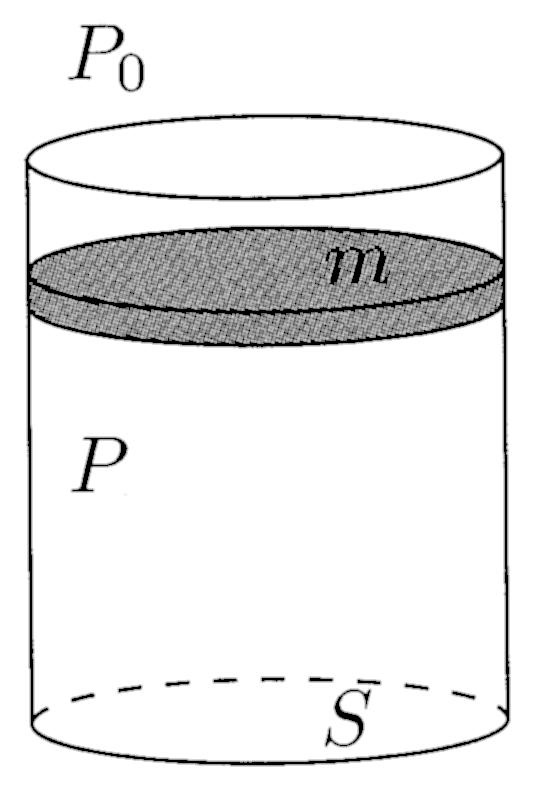
\includegraphics[keepaspectratio,width=26mm]{fig/ch14_ex1_cyl.png}\\[4mm]
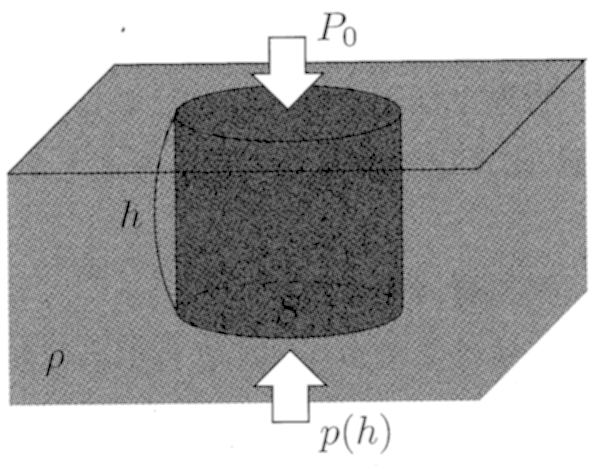
\includegraphics[keepaspectratio,width=42mm]{fig/ch14_ex1_water.png}
\end{zuright}
\end{reidai}

\begin{sisinE}
(1)は，ピストンにはたらく力のつり合いから中の気体の圧力を求める．気体の圧力を問われたら，その気体が押している面についての力のつり合いを考えるのであった．(4)も全く同じ考え方で，図の水柱についての力のつり合いを立てればよい．

(2)は分子量と物質量の関係，(3)は絶対温度とセルシウス温度の関係を使うだけである．
\end{sisinE}

\Key{$F=PS$\quad $N=nN_A$\quad $T=t+273.15$\quad 分子量$M$}

\begin{kaitou}
\begin{komon}
\ko{1} ピストンにはたらく力のつり合いより，
       \[PS=P_0S+mg\]
       よって，封入されている気体の圧力は，
       \[P=P_0+\frac{mg}{S}\U{Pa}\Ans\]
       また，シリンダーの底面が気体から受ける力は，$F=PS$より，
       \Ana{F=P_0S+mg\U{N}\Ans}
\ko{2} 窒素の分子量が28であるから，$\mathrm{N_2}$は1[mol]あたり$28\U{g}$である．よって$56\U{g}$の物質量は，
       \[n=\frac{56}{28}=2.0\U{mol}\]
       したがって分子数は，
       \Ana{\begin{aligned}
         N&=nN_{\mathrm{A}}=2.0\times 6.02\times 10^{23}\\
          &\fallingdotseq 1.2\times 10^{24}\,\text{[個]}\Ans
       \end{aligned}}
\ko{3} $T=t+273.15$より，
       \Ana{t=77-273.15=-196.15\fallingdotseq -196\Cel\Ans}
\ko{4} 図の水柱（断面積$S\U{m^2}$，高さ$h\U{m}$）にはたらく力は，上面を押す大気からの力$P_0S\U{N}$，水柱自身の重力$\rho hSg\U{N}$，下面を押し上げる力$p(h)S\U{N}$である．水柱は静止しているのでこれらがつり合い，
       \[p(h)S=P_0S+\rho hSg\]
       よって，
       \Ana{p(h)=P_0+\rho gh\U{Pa}\Ans}
\end{komon}
\end{kaitou}
\end{reidaiunit}
 
\subsection{気体の状態方程式}

体積$V[{\rm m^3}]$の容器に$n$[mol]の気体が均一に拡散しているとき，この気体の圧力を$P$[Pa]，気体の絶対温度を$T$[K]とすると，
\[\mbox{\boldmath $PV=nRT$}\]
という関係が，気体の種類によらず成立することが知られている．
これを{\bf 状態方程式}といい，比例定数$R[{\rm J/mol・K}]$を{\bf 気体定数}という．
実験により，気体定数の値は次の値をとることが知られている．
\[R=8.314[{\rm J/mol・K}] \]

この状態方程式は実在する気体全てについてほぼ成立するが，厳密には当てはまらないことが知られている．
実際にの気体は体積を持つこと，また気体分子間に相互作用（引力）が働くことが主な原因である．
この状態方程式が厳密に成立する気体を{\bf 理想気体}と呼ぶ．
理想気体であるための条件は，
\[ \MARU{1} 気体分子の体積が0[{\rm m^3}]である\]
\[ \MARU{2} 気体分子同士の相互作用がない\]
の2つである．
精密さを要求されない場合はこの状態方程式を用いてよい．
実在気体の場合でも，低圧，高温になると理想気体に近づく．

状態方程式を使う問題では，{\bf 変化の前と後のそれぞれについて状態方程式を立て，2式を組み合わせて未知の量を消去する}のが基本である．
このとき，変化の前後で値の変わらない量（物質量$n$や気体定数$R$，一定に保たれている圧力・体積・温度）を式の同じ側にまとめておくと計算が楽になる．
例えば温度が一定に保たれる変化なら$PV=nRT=$（一定）であるから，$PV$の値が変化しないことがすぐに分かる．

また，二つの容器が細い管でつながれている場合には，次の2点に注意する．
\[ \MARU{1} 気体が流れていなければ，両方の容器の気体の圧力は等しい \]
\[ \MARU{2} 容器の間で気体が移動しても，全体の物質量は変わらない \]
\MARU{1}は，左右に圧力差があると気体が流れてしまうことによる．
\MARU{2}は物質量の保存であり，コックを開いたあとの圧力を求める際にはこの関係を用いる．
なお，つながれた二つの容器の{\bf 温度が等しいとは限らない}．
温度が違う場合は全体をひとまとめにできないので，容器ごとに状態方程式を立てて物質量の和を考える．

\begin{matome}{状態方程式}
 \hspace{3mm} $PV=nRT$\\
\hspace{3mm} 変化の前後で状態方程式を立てて組み合わせる\\
\hspace{3mm} つながれた容器\hspace{5mm} 圧力は等しい／全体の物質量は保存する
\end{matome}

\begin{reidaiunit}
\begin{reidai}{状態方程式}
\begin{zuright}{42mm}
\hspace{1zw}容積$V_{\mathrm{A}}$, $V_{\mathrm{B}}\U{m^3}$の容器$\mathrm{A}$，$\mathrm{B}$が，図のようにコックを持つ細い管でつながっている．最初コックは閉じられており，温度$T\U{K}$の理想気体を$\mathrm{A}$，$\mathrm{B}$それぞれに圧力が$P_{\mathrm{A}}$, $P_{\mathrm{B}}\U{Pa}$となるだけ封入した．細管の部分の体積および容器の熱膨張は無視し，気体定数を$R\U{J/mol\cdot K}$として以下の問に答えよ．
\begin{komon}
\ko{1} $\mathrm{A}$，$\mathrm{B}$それぞれの中に含まれる理想気体の物質量$n_{\mathrm{A}}$, $n_{\mathrm{B}}\U{mol}$をそれぞれ求めよ．
\ko{2} 次に，温度を$T\U{K}$に保ったままコックを開いた．このときの容器内の圧力$P\U{Pa}$を求めよ．
\ko{3} (2)において，$\mathrm{A}$から$\mathrm{B}$へ移動した理想気体の物質量$\Delta n\U{mol}$を求めよ．
\ko{4} コックを開いたままの状態で，$\mathrm{A}$の温度を$T_{\mathrm{A}}\U{K}$，$\mathrm{B}$の温度を$T_{\mathrm{B}}\U{K}$に保った．このときの容器の圧力$P'\U{Pa}$を求めよ．
\end{komon}
\zusep
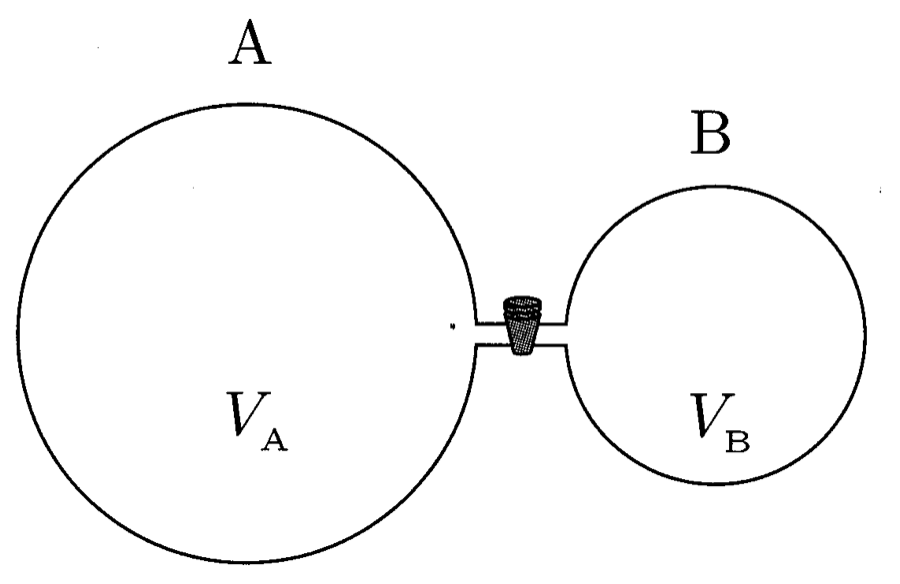
\includegraphics[keepaspectratio,width=42mm]{fig/ch14_ex2_cock.png}
\end{zuright}
\end{reidai}

\begin{sisinE}
コックを開く前と後のそれぞれについて状態方程式を立て，組み合わせればよい．コックを開いたあとは$\mathrm{A}$と$\mathrm{B}$の気体の圧力が等しくなること，そして$\mathrm{A}$，$\mathrm{B}$を合わせた全体の物質量が変わらないことがカギである．

(2)は$\mathrm{A}$と$\mathrm{B}$の温度が同じなので，$\mathrm{A}+\mathrm{B}$を体積$V_{\mathrm{A}}+V_{\mathrm{B}}$の一つの容器とみなしてよい．一方(4)では$\mathrm{A}$と$\mathrm{B}$の温度が違うのでひとまとめにできない．容器ごとに状態方程式を立て，物質量の和が変わらないことを使う．

左右に圧力差があると気体が流れる．すなわち{\bf 気体が流れていないとき左右の圧力は同じ}である．
\end{sisinE}

\Key{状態方程式\quad $PV=nRT$}


\begin{kaitou}
\begin{komon}
\ko{1} コックを開く前の$\mathrm{A}$，$\mathrm{B}$について状態方程式を立てると，
       \[\mathrm{A}:P_{\mathrm{A}}V_{\mathrm{A}}=n_{\mathrm{A}}RT\Eq{1}\]
       \[\mathrm{B}:P_{\mathrm{B}}V_{\mathrm{B}}=n_{\mathrm{B}}RT\Eq{2}\]
       よって，
       \Ana{n_{\mathrm{A}}=\frac{P_{\mathrm{A}}V_{\mathrm{A}}}{RT}\U{mol}, \quad n_{\mathrm{B}}=\frac{P_{\mathrm{B}}V_{\mathrm{B}}}{RT}\U{mol}\Ans}
\ko{2} コックを開くと$\mathrm{A}$と$\mathrm{B}$の気体の圧力は等しくなる．また，全体の物質量は$n_{\mathrm{A}}+n_{\mathrm{B}}$のまま変わらず，温度も$T$のままである．よって$\mathrm{A}+\mathrm{B}$を体積$V_{\mathrm{A}}+V_{\mathrm{B}}$の一つの容器とみなして状態方程式を立てると，
       \[P(V_{\mathrm{A}}+V_{\mathrm{B}})=(n_{\mathrm{A}}+n_{\mathrm{B}})RT\]
       \MARU{1}\MARU{2}を代入して，
       \Ana{P=\frac{P_{\mathrm{A}}V_{\mathrm{A}}+P_{\mathrm{B}}V_{\mathrm{B}}}{V_{\mathrm{A}}+V_{\mathrm{B}}}\U{Pa}\Ans\Eq{3}}
\ko{3} コックを開いた後の$\mathrm{A}$内の物質量を$n_{\mathrm{A}}'\U{mol}$とすると，$\mathrm{A}$についての状態方程式より，
       \[PV_{\mathrm{A}}=n_{\mathrm{A}}'RT\]
       $\mathrm{A}$から$\mathrm{B}$へ移動した物質量は$\Delta n=n_{\mathrm{A}}-n_{\mathrm{A}}'$であるから，\MARU{1}\MARU{3}より，
       \[\Delta n=\frac{(P_{\mathrm{A}}-P)V_{\mathrm{A}}}{RT}=\frac{V_{\mathrm{A}}V_{\mathrm{B}}(P_{\mathrm{A}}-P_{\mathrm{B}})}{RT(V_{\mathrm{A}}+V_{\mathrm{B}})}\U{mol}\]
       \hspace*{\fill}\Ans
\ko{4} $\mathrm{A}$と$\mathrm{B}$は細管でつながれているので圧力は等しく$P'\U{Pa}$である．一方，温度は$\mathrm{A}$が$T_{\mathrm{A}}$，$\mathrm{B}$が$T_{\mathrm{B}}$と異なるので，それぞれについて状態方程式を立てる．このときの$\mathrm{A}$，$\mathrm{B}$内の物質量を$n_{\mathrm{A}}''$, $n_{\mathrm{B}}''\U{mol}$とすると，
       \[\mathrm{A}:P'V_{\mathrm{A}}=n_{\mathrm{A}}''RT_{\mathrm{A}}\]
       \[\mathrm{B}:P'V_{\mathrm{B}}=n_{\mathrm{B}}''RT_{\mathrm{B}}\]
       \hspace{1zw}全体の物質量は変わらないので，
       \[n_{\mathrm{A}}''+n_{\mathrm{B}}''=n_{\mathrm{A}}+n_{\mathrm{B}}\]
       すなわち\MARU{1}\MARU{2}より，
       \[\frac{P'V_{\mathrm{A}}}{RT_{\mathrm{A}}}+\frac{P'V_{\mathrm{B}}}{RT_{\mathrm{B}}}=\frac{P_{\mathrm{A}}V_{\mathrm{A}}+P_{\mathrm{B}}V_{\mathrm{B}}}{RT}\]
       よって，
       \Ana{P'=\frac{(P_{\mathrm{A}}V_{\mathrm{A}}+P_{\mathrm{B}}V_{\mathrm{B}})T_{\mathrm{A}}T_{\mathrm{B}}}{T(V_{\mathrm{A}}T_{\mathrm{B}}+V_{\mathrm{B}}T_{\mathrm{A}})}\U{Pa}\Ans}
\end{komon}
\end{kaitou}
\end{reidaiunit}
 
\subsection{熱とエネルギー}

世の中にある物質は原子，分子によって構成されているが，熱は物質を構成している原子・分子の運動に基づく{\bf エネルギーの一つの形態}であり，熱いというのはその運動が激しい状態に対応し，冷たいというのは運動が少ない状態に対応している．
例えば，熱いものを触ったときに熱いと感じるのは，原子・分子が激しく運動してぶつかってくるのが原因である．
このように，熱や温度というのは物体の構成原子・分子の微細な運動と密接に関係している．

\begin{wrapfigure}[10]{r}[5mm]{70mm}
  \centering
  \vspace{-5mm}
  
\includegraphics[keepaspectratio,width=70mm]
  {text_p66_fig1.png}
\end{wrapfigure}
熱い物体Aと冷たい物体Bを接触させたときには，Aの温度は下がり，Bの温度は上がるが，これは接触部分での原子・分子の衝突を通してAの原子・分子の運動がBの原子・分子の運動へと移っていくからである．
この現象を，{\bf AからBへ熱が移った}と表現する．

このように熱は本質的には構成原子・分子の微細な運動エネルギーによるものであるから，移動した熱の量はエネルギーの単位[J]を用いて表すことができる．
しかし，通常の熱の移動現象を扱う際には日常生活に密接した単位である{\bf カロリー[cal]}を用いられることも多い．
{\bf 1[cal]は水1[g]の温度を1[K]だけ高めるのに必要な熱量}として定義される．
カロリーとジュールの間には，1[cal]=4.186[J]の関係がある．
この換算率を{\bf 熱の仕事当量}という．
\[ J \fallingdotseq 4.2[{\rm J/cal}] \]

一般の物質の熱しやすさ・冷めやすさは比熱によって表す．
物質1[g]あたりの温度を1[K]上げるのに必要な熱量を{\bf 比熱}\mbox{\boldmath $c$}{\bf [cal/g・K]}という．
比熱を用いると，その物質を温度上昇させるのに必要な熱量が求められる．
その物質の比熱を$c$[cal/g・K]，質量を$m$[g]，上昇させる温度を$\Delta T$[K]とすると，必要な熱量$Q$[cal]は
\[ \mbox{\boldmath $Q=mc\Delta T$} \hspace{2mm} [{\rm cal}] \]
と求められる．

また，ある物体の温度を1[K]上げるのに必要な熱量を{\bf 熱容量}\mbox{\boldmath $C$}{\bf [cal/K]}という．
$C=mc$なる関係式が成立するので，この物体の温度を$\Delta T$[K]だけ上昇させるには，
\[ \mbox{\boldmath $Q=C\Delta T$} \hspace{2mm} [{\rm cal}]\]
だけの熱量が必要である．

温度の異なる二つの物体を接触させると，高温の物体から低温の物体へと熱が移動する．
やがて両者の温度が等しくなると熱の移動は止まる．
この状態を{\bf 熱平衡状態}という．

外部との熱のやり取りがなければ，{\bf 高温の物体が失った熱量と，低温の物体が得た熱量は等しい．}
これを{\bf 熱量の保存}という．
熱平衡状態の温度を文字でおいて，
\[ \mbox{\boldmath （高温の物体が失った熱量）＝（低温の物体が得た熱量）} \]
の形の式を立てれば，その温度が求められる．

このとき，{\bf 液体を入れてある容器も液体と一緒に温度が変わる}ことを忘れてはならない．
容器の熱容量が$C$[cal/K]と与えられていれば，容器が得た熱量として$C\Delta T$[cal]を右辺に加える必要がある．

\begin{matome}{熱の仕事当量・比熱・熱容量}
 \hspace{3mm} $J \fallingdotseq 4.2$\hspace{2mm}[J/cal]\\
\hspace{3mm} $Q=mc\Delta T$\hspace{2mm}[cal]\hspace{10mm} 比熱$c$\hspace{2mm}[cal/g・K]\\
\hspace{3mm} $Q=C\Delta T$\hspace{2mm}[cal]\hspace{13mm} 熱容量$C$\hspace{2mm}[cal/K]\\
\hspace{3mm} 熱量の保存\hspace{9mm} （高温の物体が失った熱量）＝（低温の物体が得た熱量）
\end{matome}

\begin{reidaiunit}
\begin{reidai}{熱の仕事当量}
\hspace{1zw}質量$500\U{g}$の金属塊を$80\Cel$に熱し，$20\Cel$の水$450\U{g}$の中に入れたところ，全体の温度は$30\Cel$となった．容器の熱容量が$50\U{cal/K}$であるとき，この金属の比熱を求めよ．
\end{reidai}

\begin{sisinE}
熱量の保存を使う．金属塊が失った熱量が，水と容器の温度上昇に使われている．{\bf 容器も水と一緒に温度が上がっている}ことを忘れないこと．なお水の比熱は$1\U{cal/g\cdot K}$である．
\end{sisinE}

\Key{$Q=mc\Delta T$\,[cal]\quad $Q=C\Delta T$\,[cal]}

\begin{kaitou}
\hspace{1zw}金属の比熱を$c\U{cal/g\cdot K}$とする．金属塊は$80\Cel$から$30\Cel$まで$50\U{K}$下がり，水と容器はともに$20\Cel$から$30\Cel$まで$10\U{K}$上がる．よって，金属塊が失った熱量$Q\U{cal}$，水が得た熱量$Q'\U{cal}$，容器が得た熱量$Q''\U{cal}$はそれぞれ，
\[Q=500\cdot c\cdot(80-30)=25000c\]
\[Q'=450\cdot 1\cdot(30-20)=4500\]
\[Q''=50\cdot(30-20)=500\]
\hspace{1zw}熱量の保存より，金属塊が失った熱量が水と容器の温度上昇に使われたので，
\[Q=Q'+Q''\]
すなわち，
\[25000c=4500+500=5000\]
よって，
\Ana{c=0.20\U{cal/g\cdot K}\Ans}
\end{kaitou}
\end{reidaiunit}
 
\subsection{熱力学第一法則}

\begin{wrapfigure}[8]{r}[5mm]{90mm}
  \centering
  \vspace{-5mm}
  
\includegraphics[keepaspectratio,width=90mm]
  {text_p67_fig1.png}
\end{wrapfigure}
熱とはエネルギーの一形態であり，物体内部に蓄えられることのできるエネルギーだとみなすことができるが，このように，物体内部に蓄えられるエネルギーのことを{\bf 内部エネルギー}と呼ぶ．
物体に対して熱や仕事といったエネルギーを与えればこの内部エネルギーを増加させることができ，逆に物体が外界に対して熱を放出したり仕事をしたりすればこの内部エネルギーは減少する．
しかし，いかなる場合であってもそのエネルギーの収支関係は必ずつり合う．
これを{\bf 熱力学第一法則}という．

例えば，ある物体に対して外から$Q_{in}$[J]の熱量と，$W_{in}$[J]の仕事を加えたとする．
この場合，これら2つが内部エネルギーの増分$\Delta U$[J]となったのであるから，熱力学第一法則は，
\[ \Delta U=Q_{in}+W_{in}\]
と表される．

内部エネルギーについては常に増加を正とした$\Delta U$で扱うが，{\bf 熱や仕事は，気体に対して加えられたものなのか，気体が外界に対して与えたものなのかが非常に重要である．}気体が外界に対してした仕事$W_{out}$との間には$W_{out}=-W_{in}$の関係が成り立つので，熱力学第一法則は上の式を変形して
\[ Q_{in} =\Delta U +W_{out}\]
の形で扱う方が良い．気体が膨張すると$W_{out}>0$，圧縮すると$W_{out}<0$となる．

\begin{matome}{熱力学第一法則}
 \hspace{3mm} 外部が気体に与えた熱量を$Q_{in}$，気体が外部にした仕事を$W_{out}$，気体の内部エネルギーの増加量を$\Delta U$とすると，
\[ Q_{in}=\Delta U +W_{out}\]
が成り立つ．
\end{matome}

問題によっては，熱や仕事が「気体が放出した熱量」「気体がされた仕事」といった{\bf 逆向き}で与えられていることがある．
その場合は公式にそのまま代入せず，まず$Q_{in}$と$W_{out}$に読み替えてから代入する．
例えば気体が外界に$q$[J]の熱量を放出したのなら$Q_{in}=-q$[J]，外界が気体に$W$[J]の仕事をしたのなら$W_{out}=-W$[J]である．
{\bf 向きを$Q_{in}$，$W_{out}$に揃えてから式に入れる}という手順を守れば符号を間違えない．
\begin{reidaiunit}
\begin{reidai}{熱力学第一法則}
\begin{komon}
\ko{1} 物体が外界に放出した熱量$q\U{J}$，物体が外界からされた仕事$W\U{J}$，物体の内部エネルギー増加$\Delta U\U{J}$の間に成り立つ熱力学第一法則の式を示せ．
\ko{2} 物体が外界に放出した熱量$q\U{J}$，物体が外界に対してした仕事$w\U{J}$，物体の内部エネルギー増加$\Delta U\U{J}$の間に成り立つ熱力学第一法則の式を示せ．
\end{komon}
\end{reidai}

\begin{sisinE}
与えられている熱量・仕事の向きが，公式の$Q_{in}$（外部が気体に与えた熱量）・$W_{out}$（気体が外部にした仕事）と逆になっている．公式にそのまま代入せず，まず$Q_{in}$と$W_{out}$に読み替えてから代入する，という手順を守ればよい．
\end{sisinE}

\Key{熱量・仕事の出入りを把握 $\Rightarrow$ 熱力学第一法則の利用}

\begin{kaitou}
\begin{komon}
\ko{1} 物体が外界に$q\U{J}$の熱量を放出したのだから，外部が物体に与えた熱量は$Q_{in}=-q\U{J}$である．また，物体が外界からされた仕事が$W\U{J}$なのだから，物体が外界にした仕事は$W_{out}=-W\U{J}$である．これらを$Q_{in}=\Delta U+W_{out}$に代入して，
       \[-q=\Delta U+(-W)\]
       よって，
       \Ana{\Delta U=-q+W\U{J}\Ans}
\ko{2} (1)と同様に$Q_{in}=-q\U{J}$である．今度は物体が外界にした仕事が$w\U{J}$なのだから，$W_{out}=w\U{J}$である．よって，
       \[-q=\Delta U+w\]
       すなわち，
       \Ana{\Delta U=-q-w\U{J}\Ans}
\end{komon}
\end{kaitou}
\end{reidaiunit}






\subsection{熱力学第二法則}

世の中の物理現象には，ある変化A$\rightarrow$Bに対して，それを完全に時間に対して逆行させることのできる変化と，それができない変化の2つがある．
前者を{\bf 可逆変化}といい，後者を{\bf 不可逆変化}という．

\begin{wrapfigure}[4]{r}[5mm]{70mm}
  \centering
  \vspace{-5mm}
  
\includegraphics[keepaspectratio,width=70mm]
  {text_p68_fig1.png}
\end{wrapfigure}
例えば図のような床面上での単振動を考えてみる．
もし床面に完全に摩擦がなく，空気抵抗もなければこの振動は永久に続き，その力学的エネルギーは一定に保たれる．
これは可逆変化である．

しかし実際には床面には必ずわずかながらの摩擦があり，空気抵抗もある．
そのため，単振動の振幅は減衰してついには止まる．
この最中に失われた力学的エネルギーは摩擦熱などとなっておもりを温めたり空気中に拡散していく．
しかしこの逆の現象，すなわち静止しているおもりが周囲から熱を自発的に吸収してひとりでに振動することは決してない．
このような変化を不可逆変化という．

また同様に，高温の物体Aと低温の物体Bとを接触させておくと，AからBへと熱が流れ，両者は等しい温度となるが，この逆の現象，すなわち等しい温度となっている2つの物体A，Bの片方からもう片方へ熱が移動し，低温の物体から高温の物体へ熱が移動することは決してない．
これも不可逆変化である．

このような，熱の発生現象や熱伝導現象は不可逆変化であるが，これらの不可逆変化の逆方向の変化はエネルギーの出入りが逆になるだけであるからエネルギー保存則に矛盾しているわけではない．
そうした不可逆反応について，どちらの方向へ進むのは可能でどちらは不可能なのかを支配しているのが{\bf 熱力学第二法則}である．

\begin{matome}{熱力学第二法則}
 \hspace{3mm} ある温度の熱源から熱を奪って自分の力学的エネルギーに変え，かつ自分と周囲のものが元の状態に戻るような変化はできない．
\end{matome}

熱力学第二法則には他にもいろいろな表現法がある．
その代表的な表現を2つ挙げる．

\Kou{1}{トムソンの原理}

熱が自発的に力学的な仕事・エネルギーに変化することはない．\\

\Kou{2}{クラウジウスの原理}

熱が低温の物体から高温の物体へ自発的に移ることはない．\\

この2つは表現こそ違うが同じ内容を述べており，対偶をとることで互いに導き合うことができる．

\newpage

%%%%%%%%%%%%%%%%%%%%  練習問題（旧 prob_p35.png / prob_p36.png）  %%%%%%%%%%%%%%%%%%%%
% 第2章（熱力学）から問題番号を［1］に振り直す（原本もここで番号がリセットされている）
\setcounter{qno}{0}

\Rank{A問題}

\Mon{基本事項の確認}

\hspace{1zw}以下の設問に答えよ．ただし，気体定数は$8.31\U{J/mol\cdot K}$である．
\begin{komon}
\ko{1} シリンダー内に断面積$1.0\times 10^{-2}\U{m^2}$のピストンで閉じ込められた気体が，$5.0\U{N}$の力でピストンを押している．この気体の圧力は何$\U{Pa}$か．有効数字2桁で求めよ．
\ko{2} 酸素気体$\mathrm{O_2}$ $96\U{g}$中に含まれている酸素分子の数は何個か．ただし，アボガドロ数を$N_{\mathrm{A}}=6.02\times 10^{23}$\,[個/mol]とする．有効数字2桁で求めよ．
\ko{3} 温度$20\Cel$の水$300\U{g}$を$100\Cel$まで加熱するのに必要な熱量は何$\U{cal}$か．またこれは何$\U{J}$か．ただし，熱の仕事当量を$J=4.2\U{J/cal}$とする．有効数字2桁で求めよ．
\ko{4} 質量$200\U{g}$の金属塊の温度を$20\Cel$から$60\Cel$まで加熱するのに要する熱量が$56000\U{cal}$であった．この金属の比熱は何$\U{cal/g\cdot K}$か．また，この金属塊の熱容量は何$\U{cal/K}$か．有効数字2桁で求めよ．
\end{komon}

\Rank{B問題}

\Mon{状態方程式}

\hspace{1zw}容器中に理想気体が入っており，圧力$p_0\U{Pa}$，体積$V_0\U{m^3}$におけるその気体の温度を$T_0\U{K}$とする．
\begin{komon}
\ko{1} 温度を$T_0\U{K}$に保ったまま，体積を$kV_0\U{m^3}$になるまで膨張したときの気体の圧力を求めよ．
\ko{2} 圧力を$p_0\U{Pa}$に保ったまま，温度が$kT_0\U{K}$になるまで加熱したときの気体の体積を求めよ．
\ko{3} 体積を$V_0\U{m^3}$に保ったまま，圧力が$kp_0\U{Pa}$になるまで熱したときの気体の温度を求めよ．
\ko{4} この気体を熱し続けて温度が$t_1\Cel$になったとき，圧力が$p_1\U{Pa}$であったとする．$0\Cel=273.15\U{K}$として，気体の体積を求めよ．
\end{komon}

\Mon[\Sitei]{状態方程式}

\begin{zuright}{47mm}
\hspace{1zw}右図のように断熱材でできた自由に動くことのできるピストン$\mathrm{C}$で，長さ$l_{\mathrm{A}}\U{m}$の$\mathrm{A}$と長さ$l_{\mathrm{B}}\U{m}$の$\mathrm{B}$の二つの部分に分けられた容器があり，$\mathrm{A}$，$\mathrm{B}$にはともに温度$T_0\U{K}$，圧力$p_0\U{Pa}$の理想気体が入っている．$\mathrm{A}$内の気体はそのままにし，$\mathrm{B}$内の気体だけを温めて温度を$T_1\U{K}$に上げて保ったところ，$\mathrm{C}$は$l\U{m}$だけ移動した．
\begin{komon}
\ko{1} $\mathrm{C}$はどちら向きへ移動するか．
\ko{2} 移動後の$\mathrm{A}$内の気体の温度および，$\mathrm{A}$，$\mathrm{B}$内の気体の圧力を求めよ．
\end{komon}
\zusep
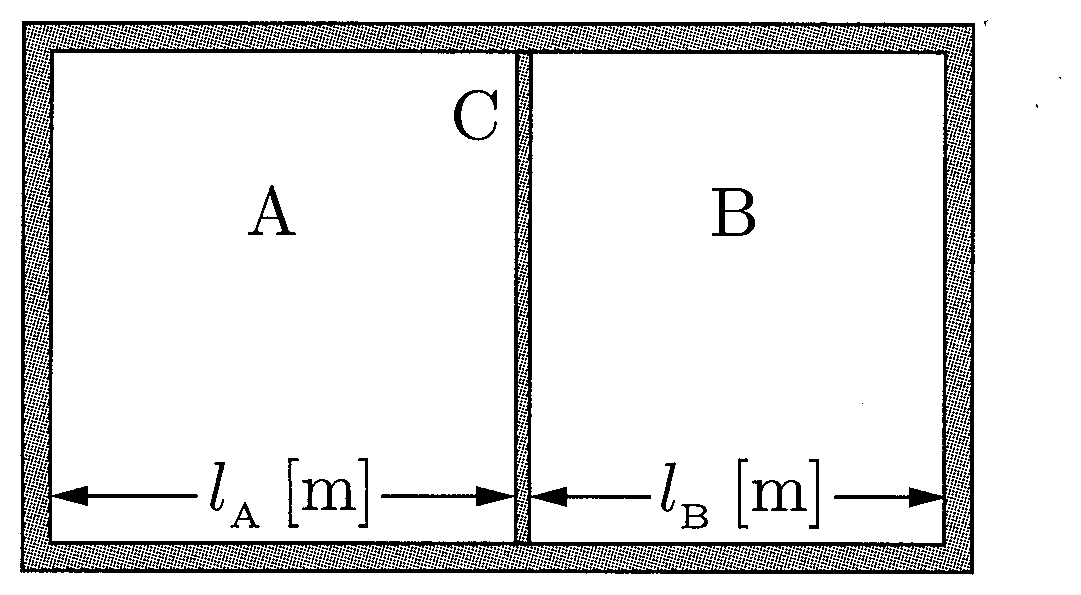
\includegraphics[keepaspectratio,width=47mm]{fig/ch14_p35_cyl.png}
\end{zuright}

\Mon[\Sitei]{熱量の保存}

\hspace{1zw}比熱$c_{\mathrm{A}}\U{cal/g\cdot K}$，質量$m_{\mathrm{A}}\U{g}$，温度$t_{\mathrm{A}}\Cel$の金属$\mathrm{A}$と，比熱$c_{\mathrm{B}}\U{cal/g\cdot K}$，質量$m_{\mathrm{B}}\U{g}$，温度$t_{\mathrm{B}}\Cel$の金属$\mathrm{B}$を接触させ十分時間が経ったところ，$\mathrm{A}$，$\mathrm{B}$間で熱のやり取りが行われ，熱平衡状態に達した．$t_{\mathrm{A}}>t_{\mathrm{B}}$として以下の問に答えよ．
\begin{komon}
\ko{1} 熱平衡状態における$\mathrm{A}$，$\mathrm{B}$の温度を求めよ．
\ko{2} このとき$\mathrm{A}$の失った熱量および$\mathrm{B}$が得た熱量を求めよ．
\end{komon}

\Mon{熱量の保存}

\hspace{1zw}質量$M\U{g}$の銅製の容器（温度$t_0\Cel$）に温度$t_0\Cel$の水が$w\U{g}$入っている．この中へ温度$t\Cel$（$t>t_0$），質量$m\U{g}$の銅球を入れてかきまぜたところ，全体の温度は一様に$t'\Cel$になった．これらを元に，銅の比熱を求めよ．
% 誤植訂正（2026-08-29）：元の問題集は「この中への温度 t[C]（t>t_0），質量 m[g] の銅球を
%   入れて」となっていたが，「この中へ温度 t[C]…の銅球を入れて」が正しい（「への」の「の」が余分）．

\Mon{摩擦熱}

\hspace{1zw}時速$72\U{km/h}$で走っている質量$1\U{t}$の自動車がブレーキをかけたところ，自動車は摩擦のため静止した．摩擦によって生じた熱量は何$\U{cal}$か．ただし熱の仕事当量を$J=4.2\U{J/cal}$とする．

\Mon{熱力学第一法則}

\hspace{1zw}ある気体が状態変化する際，気体に外界から加えられた熱量，気体の内部エネルギーの増加量，そして気体が外界に対してした仕事がそれぞれ$Q\U{J}$，$\Delta U\U{J}$，$W\U{J}$であった．これについて以下の問に答えよ．
\begin{komon}
\ko{1} $Q$, $\Delta U$, $W$の間に成り立つ熱力学第一法則を記せ．
\end{komon}
\hspace{1zw}またこの状態変化の際の仕事・熱のやり取りを，気体が熱を外界に放出し，気体が外界から仕事をされたとして捉え，それぞれの量を$Q'\U{J}$，$W'\U{J}$とおく．
\begin{komon}
\ko{2} $Q'$, $\Delta U$, $W'$の間に成り立つ関係式を求めよ．
\end{komon}

\Rank{C問題}

\Mon{状態方程式}

\begin{zuright}{41mm}
\hspace{1zw}図のように容積の等しい二つの容器$\mathrm{A}$，$\mathrm{B}$が細管でつながれ，コック$\mathrm{C}$を通して温度$T_1\U{K}$，圧力$P_1\U{Pa}$の大気に通じている．はじめコック$\mathrm{C}$は開かれており，容器および内部の気体の温度はすべて大気と同じ温度であった．細管の容積と容器の熱膨張を無視し，空気は理想気体とみなしてよいものとして以下の問に答えよ．
\zusep
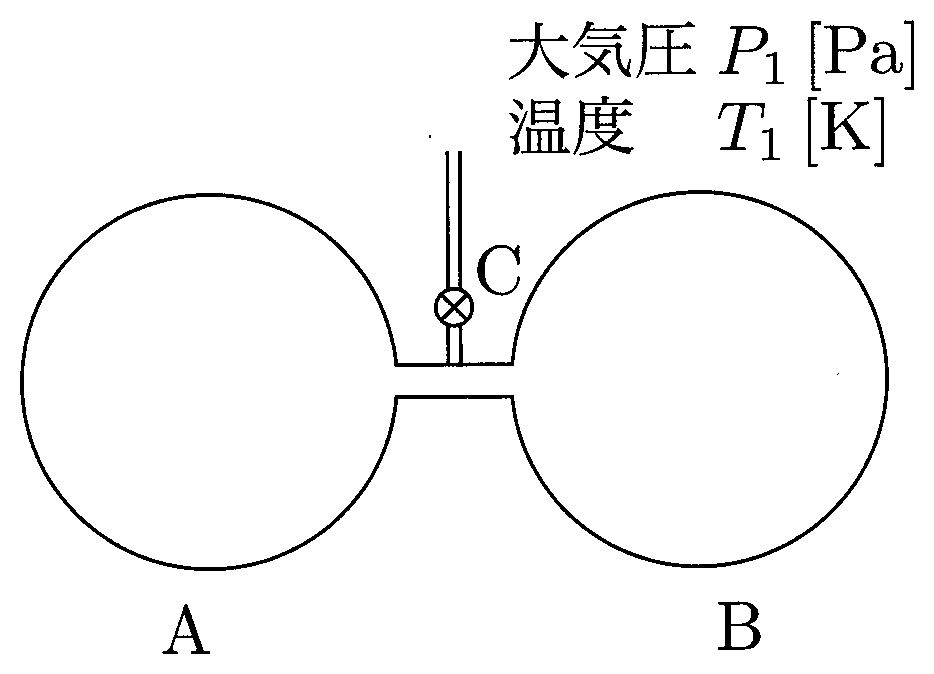
\includegraphics[keepaspectratio,width=41mm]{fig/ch14_p36_flask.png}
\end{zuright}
\vspace{-\medskipamount}
\begin{komon}
\ko{1} コック$\mathrm{C}$を開いたまま，$\mathrm{B}$は大気と同じ温度に保ちつつ$\mathrm{A}$の温度を$T_0\U{K}$になるまでゆっくりと冷やした．$\mathrm{A}$を冷やしている間に$\mathrm{A}$，$\mathrm{B}$に流入した気体のモル数は，はじめ$\mathrm{B}$の中にあった空気のモル数の何倍か．
\ko{2} 次にコック$\mathrm{C}$を閉じ，$\mathrm{A}$をゆっくりと温めて，$\mathrm{A}$および$\mathrm{B}$の温度を再び大気の温度に等しくした．このときの$\mathrm{A}$，$\mathrm{B}$内の空気の圧力$P_2\U{Pa}$を求めよ．
\end{komon}

\Mon{熱力学第二法則}

\hspace{1zw}次の文の空欄に当てはまる語を下記の語群の中から選び，その記号で答えよ．ただし，重複して用いてもよいものとする．

\hspace{1zw}熱力学第二法則は，\framebox[3zw]{ア}変化に関係した法則で，さまざまな表現の仕方がある．
\begin{quote}
\noindent $\mathrm{I}$\hspace{2zw}クラウジウスの原理\par
\hspace{2zw}他に影響を与えないで，熱を\framebox[3zw]{イ}温の物体から\framebox[3zw]{ウ}温の物体に移すことはできない．\par
\noindent $\mathrm{I\!I}$\hspace{2zw}トムソンの原理\par
\hspace{2zw}与えられた\framebox[3zw]{エ}をすべて\framebox[3zw]{オ}に変えてしまうような熱機関をつくることはできない．
\end{quote}
\hspace{1zw}$\mathrm{I}$と$\mathrm{I\!I}$は，同じ内容を違う表現で述べてあるにすぎない．同値であることは，数学でよく用いられる対偶法によって証明することができる．これを考えてみよう．

\hspace{1zw}もし，$\mathrm{I\!I}$が成り立たないとすると，\framebox[3zw]{カ}温の熱源からもらった熱をすべて\framebox[3zw]{キ}に変えることができるから，これを\framebox[3zw]{ク}温の熱源に与えれば\framebox[3zw]{ケ}を与えたのと同じことになるので，他に影響を与えないで熱が\framebox[3zw]{コ}温の物体から\framebox[3zw]{サ}温の物体に移ったことになり，$\mathrm{I}$が否定されてしまう．同様に$\mathrm{I}$が成り立たないとすると，$\mathrm{I\!I}$が否定されるので，$\mathrm{I}$と$\mathrm{I\!I}$とは同値の関係にあると言える．

\begin{bsHosoku}{選択肢}
\noindent\hspace*{1zw}A\hspace{1zw}熱\hfill B\hspace{1zw}仕事\hfill C\hspace{1zw}高\hfill D\hspace{1zw}低\hfill E\hspace{1zw}可逆\hfill F\hspace{1zw}不可逆\hspace*{1zw}
\end{bsHosoku}

\newpage

%%%%%%%%%%%%%%%%%%%%  解答（旧 prob_p117〜p120_1.png）  %%%%%%%%%%%%%%%%%%%%
% 回タイトルは段組の“外”で出す（2.5ptの罫をページ全幅に引くため）
\KaiTitle{第14回　気体の状態方程式・熱力学第一法則}

\setlength{\columnseprule}{0.4pt}
\begin{multicols}{2}
\raggedcolumns

\Rank{A問題}
\MonN{1}{基本事項の確認}
\begin{saikei}
圧力，酸素分子の数，水の加熱に必要な熱量，金属の比熱と熱容量を求める．
\end{saikei}
\begin{sisin}
状態方程式$PV=nRT$や圧力と力の関係式$F=PS$などの関係式を利用せよ．
\end{sisin}
\begin{kaitou}
\begin{komon}
\ko{1} $P=\dfrac{F}{S}=\dfrac{5.0}{1.0\times 10^{-2}}=5.0\times 10^2\U{Pa}$\Ans
\ko{2} $\mathrm{O_2}$の分子量は$M=32\U{g/mol}$なので，$96\U{g}$は$n=\dfrac{w}{M}=\dfrac{96}{32}=3.0\U{mol}$に相当．よって，分子数は
       \[\begin{aligned}
         N&=n\cdot N_{\mathrm{A}}=3.0\times 6.02\times 10^{23}\\
          &\fallingdotseq 1.8\times 10^{24}\,\text{[個]}\Ans
       \end{aligned}\]
\ko{3} 水の比熱は$1\U{cal/g\cdot K}$であるから，
       \[\begin{aligned}
         Q&=mc\Delta t=300\cdot 1\cdot(100-20)\\
          &=2.4\times 10^4\U{cal}
       \end{aligned}\]
       また，$1\U{cal}=4.2\U{J}$なので，
       \[Q=2.4\times 10^4\times 4.2\U{J}\fallingdotseq 1.0\times 10^5\U{J}\Ans\]
\ko{4} $Q=mc\Delta t$より，$56000=200\times c\times(60-20)$が成り立つから，
       \[c=\frac{56000}{200\cdot(60-20)}=7.0\U{cal/g\cdot K}\]
       また，熱容量は，
       \[\begin{aligned}
         C&=m\cdot c=7.0\times 200\\
          &=1.4\times 10^3\U{cal/K}\Ans
       \end{aligned}\]
\end{komon}

\end{kaitou}
\Rank{B問題}
\MonN{2}{状態方程式}
\begin{saikei}
圧力$p_0$，体積$V_0$，温度$T_0$の理想気体について，等温・等圧・等積の各変化後の量を求める．
\end{saikei}
\begin{sisin}
状態方程式$PV=nRT$を元にして考える．ある量を固定して他の量を変化させる場合には，左辺もしくは右辺に変化しない量をまとめてしまうのがコツである．例えば(2)の変化では，気体の圧力が一定なので，状態方程式で一定の量の$n$, $R$, $p$を右辺にまとめると，$\dfrac{V}{T}=\dfrac{nR}{p}=$（一定）となり，$\dfrac{V}{T}$が変化していないことが分かる．
\end{sisin}
\begin{kaitou}
\hspace{1zw}気体が$n\U{mol}$あるとする．また，気体定数を$R\U{J/mol\cdot K}$とする．
\begin{komon}
\ko{1} この状態変化では気体の温度が一定であるから，理想気体の状態方程式の$n$, $R$, $T$が一定に保たれる．よって状態方程式より，$pV=nRT=$（一定）となる．変化後の気体の圧力を$p'\U{Pa}$とすれば，
       \[p'\cdot kV_0=p_0\cdot V_0\]
       ゆえに，
       \[p'=\frac{1}{k}p_0\U{Pa}\Ans\]
\ko{2} この状態変化では気体の圧力が一定であるから，理想気体の状態方程式の$n$, $R$, $p$が一定に保たれる．よって状態方程式より，$\dfrac{V}{T}=\dfrac{nR}{p}=$（一定）となる．変化後の気体の体積を$V'\U{m^3}$とすれば，
       \[\frac{V'}{kT_0}=\frac{V_0}{T_0}\]
       ゆえに，
       \[V'=kV_0\U{m^3}\Ans\]
\ko{3} この状態変化では気体の体積が一定であるから，理想気体の状態方程式の$n$, $R$, $V$が一定に保たれる．よって状態方程式より，$\dfrac{p}{T}=\dfrac{nR}{V}=$（一定）となる．変化後の気体の温度を$T'\U{K}$とすれば，
       \[\frac{kp_0}{T'}=\frac{p_0}{T_0}\]
       ゆえに，
       \[T'=kT_0\U{K}\Ans\]
\ko{4} この状態変化においては圧力，体積，温度が変化するので状態方程式をそのまま利用する．始めの状態の状態方程式は，
       \[p_0V_0=nRT_0\]
       変化後の状態方程式は，絶対温度が$t_1+273.15\U{K}$であることに注意して，変化後の体積を$V_1\U{m^3}$とすると，
       \[p_1V_1=nR(t_1+273.15)\]
       以上2式から$n$, $R$を消して$V_1$を求めると，
       \[V_1=\frac{p_0(t_1+273.15)}{p_1T_0}V_0\U{m^3}\Ans\]
\end{komon}
\end{kaitou}
\begin{chuu}
\hspace{1zw}上の解答では状態方程式を変形することで答えを導いたが，(4)と同様に，変化前・変化後の二つの状態方程式から答えを導いてもよい．例えば(2)であれば，変化前の状態方程式$p_0V_0=nRT_0$と，変化後の状態方程式$p_0V'=nR(kT_0)$の二つの組み合わせから，$V'=kV_0\U{m^3}$を導くことが可能である．
\end{chuu}

\MonN{3}{状態方程式}
\begin{saikei}
断熱ピストン$\mathrm{C}$で二分された容器．$\mathrm{B}$だけを$T_1$に温めたときの$\mathrm{C}$の移動の向き，$\mathrm{A}$の温度，$\mathrm{A}$，$\mathrm{B}$の圧力を求める．
\end{saikei}
\begin{sisin}
ピストン$\mathrm{C}$は$\mathrm{A}$，$\mathrm{B}$の気体から圧力を受けるが，例えば$\mathrm{A}$からの圧力の方が大きければピストンは右へ移動する．よって，ピストンが静止しているときは$\mathrm{A}$，$\mathrm{B}$の圧力は等しい．また，$\mathrm{C}$は断熱材であるから，$\mathrm{A}$，$\mathrm{B}$の温度は等しくなくてもよい．

本問のような問題では，変化前・変化後の気体の状態方程式を立てて考えるのが基本である．問題文では状態方程式を立てるのに必要な変数がすべて与えられていないので，適宜仮定した上で状態方程式を立てよう．
\end{sisin}
\begin{kaitou}
\hspace{1zw}ピストン$\mathrm{C}$の断面積を$S\U{m^2}$，$\mathrm{A}$，$\mathrm{B}$内の気体の物質量を$n_{\mathrm{A}}\U{mol}$，$n_{\mathrm{B}}\U{mol}$とし，気体定数を$R\U{J/mol\cdot K}$とすると，最初の状態についての状態方程式より，
\[\mathrm{A}:p_0(Sl_{\mathrm{A}})=n_{\mathrm{A}}RT_0\Eq{1}\]
\[\mathrm{B}:p_0(Sl_{\mathrm{B}})=n_{\mathrm{B}}RT_0\Eq{2}\]
である．
\begin{komon}
\ko{1} $\mathrm{B}$内の気体の温度を上げると，$\mathrm{B}$内の気体の圧力の方が$\mathrm{A}$内の気体の圧力より大きくなってしまうので，ピストン$\mathrm{C}$は$\mathrm{B}$から$\mathrm{A}$の向きへ移動する．\Ans
\ko{2} ピストン$\mathrm{C}$は自由に動くことができるので，ピストン$\mathrm{C}$が移動して静止した時の$\mathrm{A}$，$\mathrm{B}$内の気体の圧力は等しい．これを$p\U{Pa}$とする．また，このときの$\mathrm{A}$内の気体の温度を$T\U{K}$とすると，変化後のシリンダーの長さがそれぞれ$l_{\mathrm{A}}-l$, $l_{\mathrm{B}}+l$になっていることに注意して，
       \[\mathrm{A}:p\cdot S(l_{\mathrm{A}}-l)=n_{\mathrm{A}}RT\Eq{3}\]
       \[\mathrm{B}:p\cdot S(l_{\mathrm{B}}+l)=n_{\mathrm{B}}RT_1\Eq{4}\]
       が成立する．これと先に立てた状態方程式を組み合わせる．\MARU{2}，\MARU{4}より，
       \[p=\frac{l_{\mathrm{B}}T_1}{(l_{\mathrm{B}}+l)T_0}p_0\U{Pa}\Ans\]
       また，\MARU{1}，\MARU{3}および$p$より，
       \[T=\frac{(l_{\mathrm{A}}-l)l_{\mathrm{B}}}{(l_{\mathrm{B}}+l)l_{\mathrm{A}}}T_1\U{K}\Ans\]
\end{komon}
\end{kaitou}
\begin{chuu}
\hspace{1zw}$\mathrm{A}$内の気体の温度が変化することに注意．
\[\mbox{「熱の出入りがない」}\]
\[=\mbox{「温度が変化しない」}\]
と考えるのは間違いである．
\end{chuu}

\MonN{4}{熱量の保存}
\begin{saikei}
温度の違う金属$\mathrm{A}$，$\mathrm{B}$を接触させたときの熱平衡温度と，やり取りした熱量を求める．
\end{saikei}
\begin{sisin}
一般的に，熱は温度の高いものから低いものへと移っていき，最終的には両者の温度が等しくなって熱の移動が止まる．この状態を「熱平衡状態」と呼ぶ．

熱量の保存より，$\mathrm{A}$が失った熱量分を$\mathrm{B}$が受け取っている．よって，熱平衡状態の温度を適当な文字でおき，$\mathrm{A}$が失った熱量と$\mathrm{B}$が得た熱量をその文字で表して考える．
\end{sisin}
\begin{kaitou}
\begin{komon}
\ko{1} 熱平衡状態における$\mathrm{A}$，$\mathrm{B}$の温度を$t\Cel$とする．この状態に至るまでに，$\mathrm{A}$の温度は$t_{\mathrm{A}}-t$だけ下がり，$\mathrm{B}$の温度は$t-t_{\mathrm{B}}$だけ上がる．よって$\mathrm{A}$が失った熱量$Q_{\mathrm{A}}\U{cal}$および$\mathrm{B}$が得た熱量$Q_{\mathrm{B}}\U{cal}$は，
       \[Q_{\mathrm{A}}=m_{\mathrm{A}}c_{\mathrm{A}}(t_{\mathrm{A}}-t),\]
       \[Q_{\mathrm{B}}=m_{\mathrm{B}}c_{\mathrm{B}}(t-t_{\mathrm{B}})\]
       \hspace{1zw}熱量の保存より，$\mathrm{A}$が失った熱量と$\mathrm{B}$が得た熱量は等しいので，
       \[m_{\mathrm{A}}c_{\mathrm{A}}(t_{\mathrm{A}}-t)=m_{\mathrm{B}}c_{\mathrm{B}}(t-t_{\mathrm{B}})\]
       である．これを解いて，
       \[t=\frac{m_{\mathrm{A}}c_{\mathrm{A}}t_{\mathrm{A}}+m_{\mathrm{B}}c_{\mathrm{B}}t_{\mathrm{B}}}{m_{\mathrm{A}}c_{\mathrm{A}}+m_{\mathrm{B}}c_{\mathrm{B}}}\Cel\Ans\]
\ko{2} (1)の$t$を$Q_{\mathrm{A}}$, $Q_{\mathrm{B}}$の式に代入して，
       \[Q_{\mathrm{A}}=Q_{\mathrm{B}}=\frac{m_{\mathrm{A}}c_{\mathrm{A}}m_{\mathrm{B}}c_{\mathrm{B}}(t_{\mathrm{A}}-t_{\mathrm{B}})}{m_{\mathrm{A}}c_{\mathrm{A}}+m_{\mathrm{B}}c_{\mathrm{B}}}\U{cal}\]
       \hspace*{\fill}\Ans
\end{komon}

\end{kaitou}
\MonN{5}{熱量の保存}
\begin{saikei}
銅製の容器・水・銅球が熱平衡に達したときの温度から，銅の比熱を求める．
\end{saikei}
\begin{sisin}
最終的に全体の温度が$t'\Cel$になったのであるから，水，銅球だけでなく容器の温度も変化している．熱の移動を考えれば，銅球が失った熱量は水，容器の温度上昇に利用されている．これを表す式を立てればよい．
\end{sisin}
\begin{kaitou}
\hspace{1zw}銅の比熱を$c\U{cal/g\cdot K}$とする．この変化にて銅球は$t-t'$だけ温度が下がり，水と容器はともに$t'-t_0$だけ温度が上がったので，銅球が失った熱量$Q\U{cal}$，水，熱量計が得た熱量$Q'\U{cal}$，$Q''\U{cal}$はそれぞれ，
\[Q=mc(t-t')\]
\[Q'=w\cdot 1\cdot(t'-t_0)\]
\hspace*{2zw}（注：水の比熱は$1\U{cal/g\cdot K}$）
% 誤植訂正（2026-08-29）：元の問題集はこの注が Q''=Mc(t'-t_0) の行に置かれていたが，
%   注が説明しているのは Q' の式に現れる「1」（水の比熱）なので Q' の行に移した．
%   Q'' は銅製の容器の式で，比熱は c であり 1 ではない．
\[Q''=Mc(t'-t_0)\]
\hspace{1zw}熱量の移動を考えると，銅球が失った熱量が，水と容器の温度上昇に利用されたので，
\[Q=Q'+Q''\]
以上をまとめると，
\[c=\frac{w(t'-t_0)}{m(t-t')-M(t'-t_0)}\U{cal/g\cdot K}\]
\hspace*{\fill}\Ans

\end{kaitou}
\MonN{6}{摩擦熱}
\begin{saikei}
$72\U{km/h}$で走る$1\U{t}$の自動車が静止するまでに生じた摩擦熱を$\U{cal}$で求める．
\end{saikei}
\begin{sisin}
自動車がブレーキをかけると摩擦力の作用により車は静止する．これをエネルギー的な観点から見ると，摩擦力によって自動車の持っていた力学的エネルギーが減少し，その減少分は熱として空気中などに散逸している．この熱を\underline{摩擦熱}という．最終的に静止したのだから，持っていた運動エネルギーすべてが摩擦熱に転化したことになる．

また運動エネルギーを求める際には，まず速さ，質量をMKS単位系に直してエネルギーを$\U{J}$単位で求めよう．
\end{sisin}
\begin{kaitou}
\hspace{1zw}ブレーキをかける前に自動車がもっていた運動エネルギーを$E\U{J}$とする．
\[1\U{t}=1000\U{kg}\]
\[72\U{km/h}=\frac{72000\U{m}}{3600\U{s}}=20\U{m/s}\]
であるから，
\[\begin{aligned}
  E&=\frac{1}{2}mv^2=\frac{1}{2}\cdot 1000\cdot 20^2\\
   &=2.0\times 10^5\U{J}
\end{aligned}\]
\hspace{1zw}摩擦によって失われた運動エネルギーはすべて摩擦熱となったので，このとき生じた熱量は$2.0\times 10^5\U{J}$である．これを$\U{cal}$単位に換算して，
\[Q=\frac{2.0\times 10^5}{4.2}\fallingdotseq 4.8\times 10^4\U{cal}\Ans\]

\end{kaitou}
\MonN{7}{熱力学第一法則}
\begin{saikei}
$Q$，$\Delta U$，$W$の間の熱力学第一法則と，熱・仕事の向きを逆にとったときの関係式を書く．
\end{saikei}
\begin{sisin}
熱力学第一法則を考える際には，熱量，仕事の出入りを把握するのが第一である．それを把握したら，簡単な図を描いてエネルギー収支を日本語で考え，それを式として表せばよい．

熱や仕事のやり取りを，気体に対して加えられたとみなして考えた場合と，気体が外界に対して放出したとみなして考えた場合とは，正負が逆になる．
\end{sisin}
\begin{kaitou}
\begin{komon}
\ko{1} 外部が気体に与えた熱量は$Q$，外部が気体にした仕事は$-W$，気体の内部エネルギーの増加量は$\Delta U$であるから，
       \[\Delta U=Q+(-W)\Ans\]
       \begin{center}
       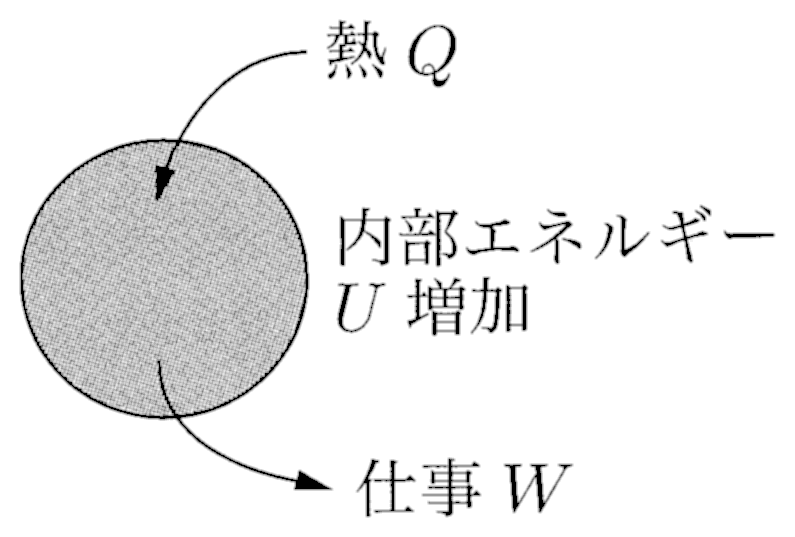
\includegraphics[keepaspectratio,width=38mm]{fig/ch14_p119_dU1.png}
       \end{center}
\ko{2} 外部が気体に与えた熱量は$-Q'$，外部が気体にした仕事は$W'$，気体の内部エネルギーの増加量は$\Delta U$であるから，
       \[\Delta U=(-Q')+W'\Ans\]
       \begin{center}
       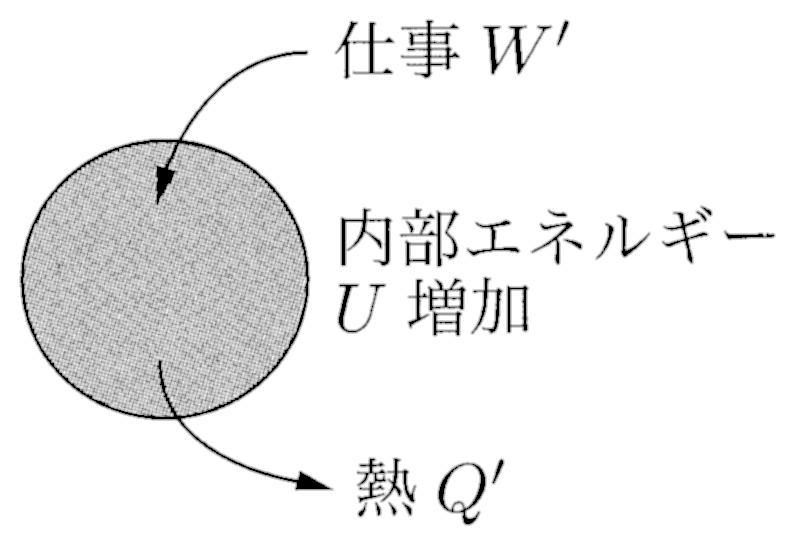
\includegraphics[keepaspectratio,width=38mm]{fig/ch14_p119_dU2.png}
       \end{center}
\end{komon}

\end{kaitou}
\Rank{C問題}
\MonN{8}{状態方程式}
\begin{saikei}
細管でつながれた容器$\mathrm{A}$，$\mathrm{B}$．$\mathrm{A}$を冷やしたときの流入モル数と，コックを閉じて温め直したときの圧力を求める．
\end{saikei}
\begin{sisin}
各状態において，各々の部分の圧力，体積，気体のモル数，温度がどのようになっているのかを考えて，$\mathrm{A}$内および$\mathrm{B}$内の状態方程式を立式し，これを整理せよ．

$\mathrm{A}$と$\mathrm{B}$は細管でつながれているが，$\mathrm{A}$と$\mathrm{B}$とに圧力差がある場合には圧力の高い方から低い方へと気体が移動してしまう．よって，\underline{定常状態においては}\hskip0pt\underline{$\mathrm{A}$と$\mathrm{B}$の}\hskip0pt\underline{気体の圧力は}\hskip0pt\underline{等しくなっている}．しかし，$\mathrm{A}$と$\mathrm{B}$との温度が等しいとは限らないことに注意．$\mathrm{A}$，$\mathrm{B}$の温度は独立に保つことができる．
\end{sisin}
\begin{kaitou}
\hspace{1zw}$\mathrm{A}$，$\mathrm{B}$の体積を$V_0\U{m^3}$，気体定数を$R\U{J/mol\cdot K}$とする．$\mathrm{A}$と$\mathrm{B}$は細管でつながれているので，常に$\mathrm{A}$，$\mathrm{B}$内の気体の圧力は等しくなっている．
\begin{komon}
\ko{1} 今，コック$\mathrm{C}$を開いているので，$\mathrm{A}$，$\mathrm{B}$内の気体の圧力は外界の圧力$P_1$に等しくなっている．この状態における$\mathrm{A}$，$\mathrm{B}$それぞれの中にある気体のモル数を$n_0\U{mol}$とすると，状態方程式より
       \[\mathrm{A},\ \mathrm{B}:P_1V_0=n_0RT_1\]
       が成立する．この状態から，コック$\mathrm{C}$を開いたまま（＝$\mathrm{A}$，$\mathrm{B}$内の気体の圧力を$P_1$に保ったまま）$\mathrm{B}$の温度を$T_1$に，$\mathrm{A}$の温度を$T_0$にした．この変化後の$\mathrm{B}$の状態方程式は
       \[\mathrm{B}:P_1V_0=n_0RT_1\]
       のまま変わらないので，$\mathrm{B}$内の気体のモル数は$n_0$のまま変わらない．変化後の$\mathrm{A}$内の気体のモル数を$n_1\U{mol}$とすると，変化後の$\mathrm{A}$の状態方程式は，
       \[\mathrm{A}:P_1V_0=n_1RT_0\]
       となる．$\mathrm{B}$内の気体のモル数は不変ゆえ$\mathrm{A}$内の気体のモル数の変化のみ考えればよく，$\mathrm{A}$を冷却していく間に流入した気体のモル数（＝$\mathrm{A}$内の気体のモル数の増加量）は，
       \[\Delta n_{\mathrm{A}}=n_1-n_0\]
       であり，これがはじめ$\mathrm{B}$内にあった気体のモル数$n_0$の何倍となるかを求めると，
       \[\frac{\Delta n_{\mathrm{A}}}{n_0}=\frac{n_1-n_0}{n_0}=\frac{n_1}{n_0}-1\]
       \[=\frac{\dfrac{P_1V_0}{RT_0}}{\dfrac{P_1V_0}{RT_1}}-1=\frac{T_1}{T_0}-1\ \mbox{[倍]}\Ans\]
\ko{2} コック$\mathrm{C}$を閉じても$\mathrm{A}$と$\mathrm{B}$は細管でつながれているので，常に$\mathrm{A}$，$\mathrm{B}$内の気体の圧力は等しくなっている．よって，変化後の$\mathrm{A}$，$\mathrm{B}$内の気体の圧力は等しい．\par
       \hspace{1zw}また$\mathrm{A}$，$\mathrm{B}$の両方を温度$T_1$にするので，$\mathrm{A}$と$\mathrm{B}$は共通の圧力，温度を持つ．よって，$\mathrm{A}$，$\mathrm{B}$内に一様にムラなく気体が分布していると考えられるので，$\mathrm{A}+\mathrm{B}$を一つの一様な系とみなして状態方程式を立てることができる．$\mathrm{A}+\mathrm{B}$の体積$2V_0$の空間に，合計$n_1+n_0$の気体分子が，圧力$P_2$，温度$T_1$で広がっているので，
       \[P_2\cdot 2V_0=(n_1+n_0)RT_1\]
       \hspace{1zw}これと(1)の状態方程式の組み合わせにより，
       \[P_2=\frac{T_0+T_1}{2T_0}P_1\U{Pa}\Ans\]
\end{komon}

\end{kaitou}
\MonN{9}{熱力学第二法則}
\begin{saikei}
クラウジウスの原理とトムソンの原理が同値であることを示す文の空欄を，語群から選んで埋める．
\end{saikei}
\begin{sisin}
誘導に従う．熱力学第二法則が入試で問われることはまずないが，熱力学第二法則の二つの代表的な表現方法であるトムソンの原理，クラウジウスの原理については頭の片隅に置いておくとよい．
\end{sisin}
\begin{kaitou}
\begin{list}{}{%
  \setlength{\leftmargin}{3zw}\setlength{\labelwidth}{1.5zw}%
  \setlength{\labelsep}{1zw}\setlength{\itemsep}{0pt}%
  \setlength{\parsep}{0pt}\setlength{\topsep}{2pt}\setlength{\partopsep}{0pt}}
\item[ア] F
\item[イ] D
\item[ウ] C（熱は自発的には高→低にしか流れない）
\item[エ] A
\item[オ] B（必ず一部分は熱を捨てる必要がある）
\item[カ] D
\item[キ] B
\item[ク] C（仕事であれば何に対してでも与えることが可能である）
\item[ケ] A（仕事も熱もエネルギーであるから，仕事という形態で高熱源にエネルギーを与えるのと，熱という形態で高熱源にエネルギーを与えるのとは何ら違いがない）
\item[コ] D
\item[サ] C
\end{list}

\end{kaitou}
\end{multicols}
